
Desenvolva um projeto que através de um potenciômetro aumente ou diminua a frequência de uma determina saída X utilizando PWM.

\section{O que é PWM ?}

A técnologia \sigla{PWM}{Pulse Width Modulation} ou no português Modulação de Largura de Pulso permite que os microcontroladores atenuem as luzes, controle a velocidade de motores e geram tensões análogicas.Isso é feito alterando o comprimento do pulso, permitidno assim a saída ser controlada.

Neste projeto iremos controlar a intesidade de brilho de um LED utilizando a \sigla{PINB0)}{saída} PWM do microncontralador: atmega8.

O pulso ocorre em uma frequência regular, neste caso na freqüência de modulação. Chamamos de \sigla{Dutty Cicle}{Ciclo de trabalho} a razão entre o tamanho do pulso pelo periodo de tempo. Logo, quanto maior é o tempo de trabalho maior também será a saída. Porntato, quando alteramos essa saída que alimenta o LED, alteramos  a intensidade do seu brilho também.

\begin{figure}[htb]
 \caption{Duty Cicle}
 \label{fig:Duty Cicle}
 \centering
 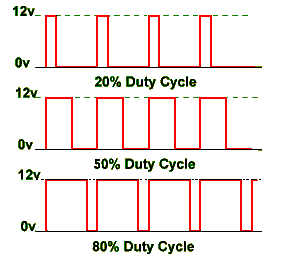
\includegraphics[scale=0.23]{Duty-Cycle.png}
 \fdireta{avrprojects:duty_cicle}
\end{figure}

\section{PWM no atmega8}

Todos os projetos aqui desenvolvidos serão utilizando o microcontrolador: ATMega8. Ele pode ser usado para gerar sinais PWM. Um microcontrolador como o ATMega8 tem três canais de hardware PWM a bordo do chip. Para o desenvolvimento deste trabalho estaremos utilizando o sinal PWM que está no pino PORTBO.

O PWM de hardware pode ser programado configurando os registradores do temporizador. O ATMega8 tem três registradores de temporizador que você precisa definir para programar o PWM:

\begin{enumerate}

\item O registrador TCCR1A deverá colocar o temporizador no modo PWM.
\item Os registradores TCNT1H e TCNT1Lsão usados para ajustar a freqüência de modulação
\item O registrador OCR1A é usado para ajustar o ciclo de trabalho.

\end{enumerate}

\section{Esquemático e Montagem}

O circuito consiste em ligar um microcontrolador ATMega8, onde que iremos ligar um LED conectador no pino PORTB0, através de um resistor de 220 ohm.

Pretendemos variar o brilho do LED através dos valores fornecidos pelo potênciometro conectado no pino PORTC0. Os valores serão lidos pela porta análogica do ATMega8, que neste caso se encontra no PORTC0.

Veja o esquematico da montagem na figura 2:

\begin{figure}[htb]
 \caption{Esquemático: Fading LED}
 \label{fig:Fading LED}
 \centering
 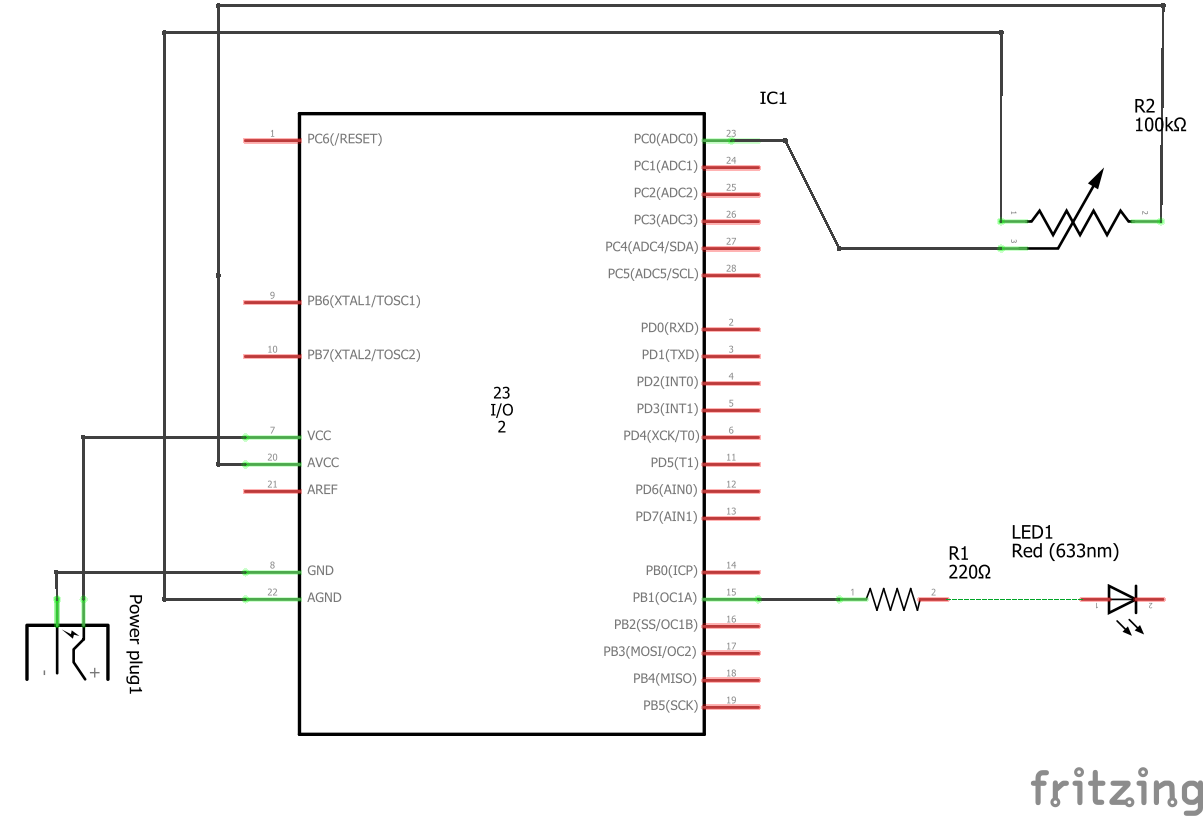
\includegraphics[scale=0.8]{esquema_fading.png}
 \fautor
\end{figure}

Veja também o circuito montado na protoboard na figura 3:

 \begin{figure}[htb]
 \caption{Montagem: Fading LED}
 \label{fig:Montagem Fading LED}
 \centering
 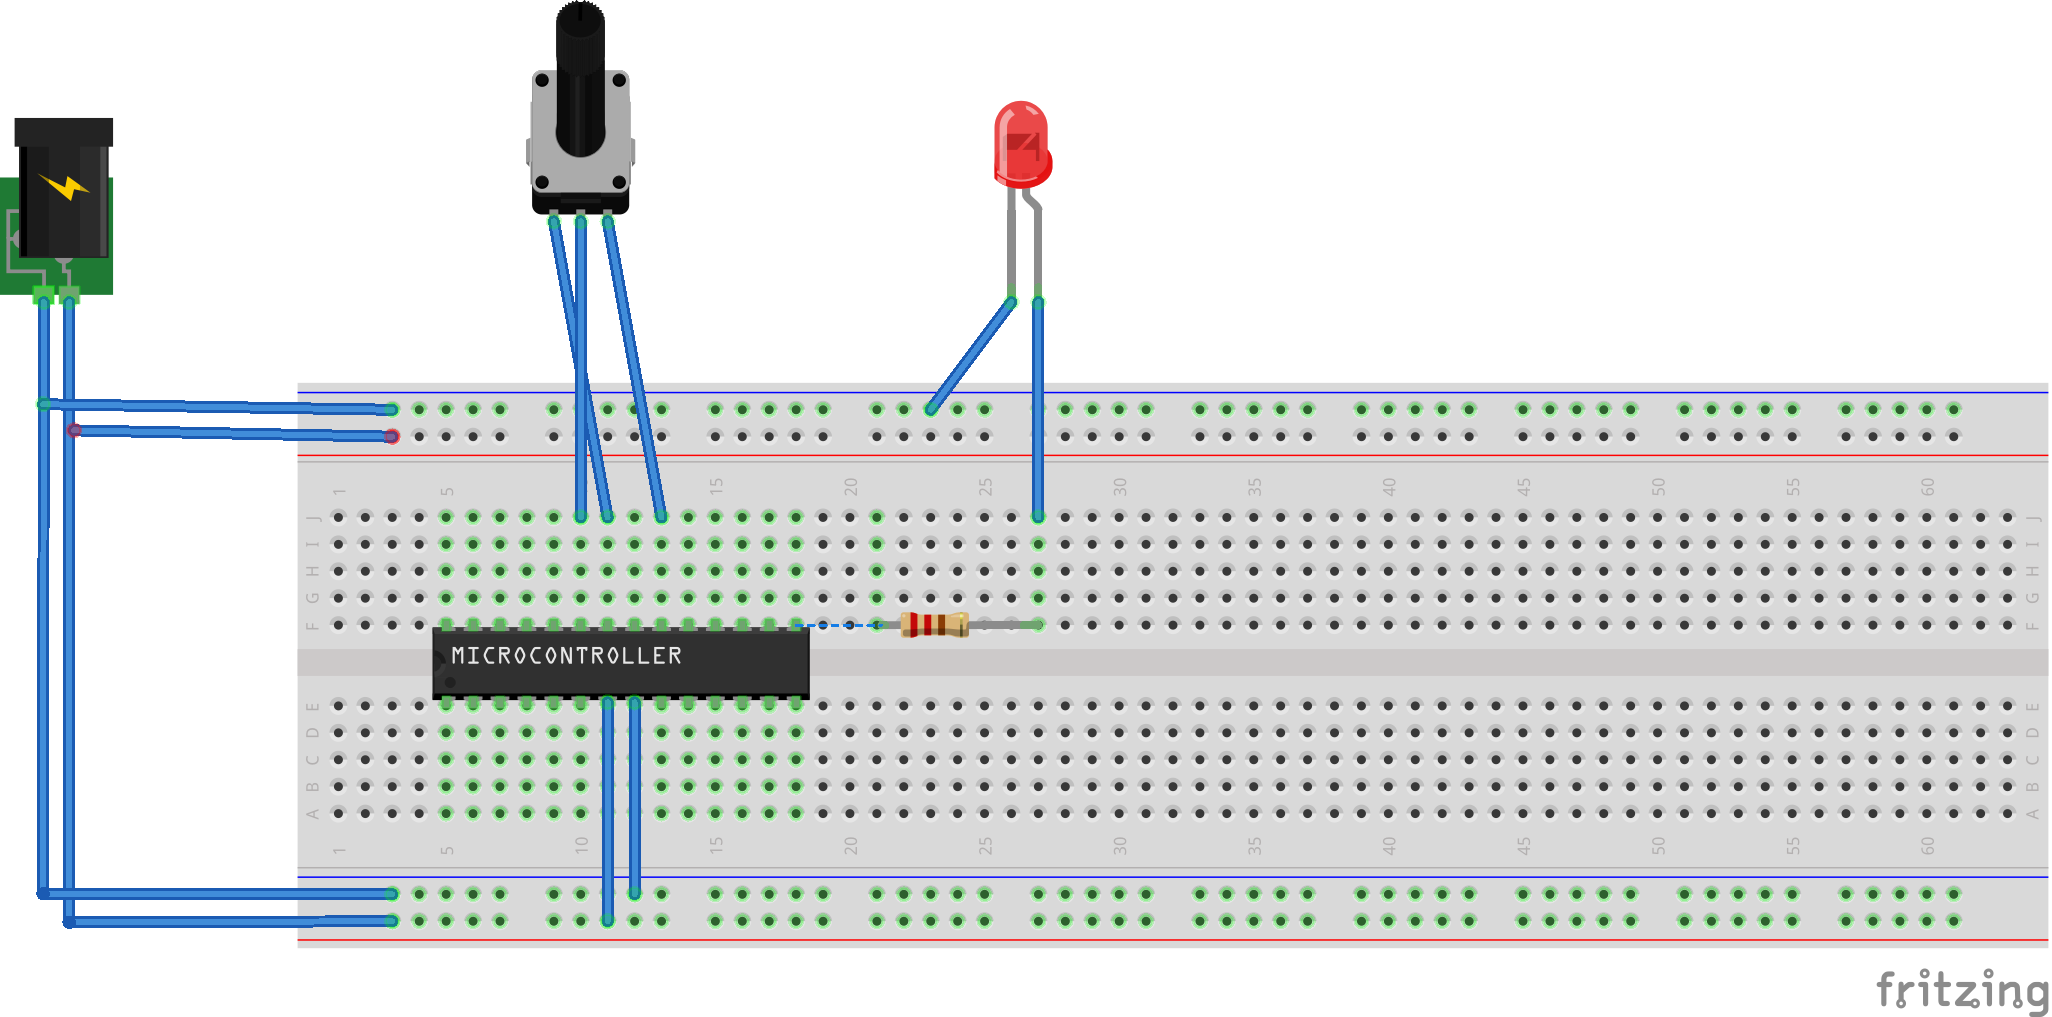
\includegraphics[scale=0.5]{montagem_fading.png}
 \fautor
\end{figure}

\section{Código em C}

%\begin{algoritmo}
%\caption{Algoritmo para cálculo de máximo divisor comum MDC($n_1$,$n_2$)}
%\label{algoritmo:mdc1}
%
% \KwIn{Dois números inteiros ($n_1, n_2$)}
% \If(\tcp*[f]{Garante que o maior número seja $n_1$}){$n_2 > n_1$}
%   {troca valores de $n_1$ e $n_2$}
% \Repeat{$r > 0$}{
%    $r \leftarrow$ resto da divisão de $n_1$ por $n_2$
%    $n_1 \leftarrow n_2$
%    $n_2 \leftarrow r$
% }
% \Return $n_1$
%\end{algoritmo}

\begin{codigo}[caption = {Fading LED}, label={codigo:fading LED},language=C, breaklines=true]
 
  /*******************************************************************
 *      Fading Led
 *
 * Universidade Federal de Goiás
 * Microcontrolador Utilizado: AVR ATMega8
 * Grupo: Marco Túlio / Vitor do Vale Bernardo / Pablo Silva
 * Descrição: O codigo recebe os valores lido na entrada PWM atráves de um/
 *		   	  Potênciometro e irá ligar o LED proporcionalmente.
 * 
 ********************************************************************/

#define FOSC 1000000UL// Clock Speed
#define BAUD 1200
#define MYUBRR ((FOSC/ (BAUD * (long)16)))

#include <avr/io.h>
#include <util/delay.h>
#include <util/setbaud.h>
#include <avr/eeprom.h>
#include <avr/interrupt.h>

void USART_Init( unsigned intubrr);
void USART_Transmit(unsigned char data);
unsigned char USART_Receive(void);
uint16_t ReadADC(uint8_t ch);
void InitADC();


int main(void)
{
	
	//PWM Initialisation
	TCCR1A = 0b10000001; // fast PWM mode 8-bit on OC1A
	TCCR1B = 0b00001010; // prescaling by 8
	
	//Initial value;
	OCR1A = 0x00;
	DDRB = 0xFF; // set port B for output


	unsigned char lei;
	InitADC();
	USART_Init(MYUBRR);
	while(1)
	{
		OCR1A =ReadADC(0);
		_delay_ms(10);
	}
}

void USART_Transmit(unsigned char data)
{
	while( !( UCSRA & (1<<UDRE)) );
	UDR = data;
}


void USART_Init(unsigned int ubrr)
{
	UBRRH=(unsigned char)(ubrr>>8);
	UBRRL=(unsigned char)ubrr;
	UCSRB=(1<<RXEN)|(1<<TXEN);
	UCSRC=(1<<URSEL)|(1<<USBS)|(3<<UCSZ0);
}

unsigned char USART_Receive(void)
{
	while(!(UCSRA & (1<<RXC)));
	return UDR;
}


void InitADC()
{
	ADMUX=(1<<REFS0);             // For Aref=AVcc;
	ADCSRA=(1<<ADEN)|(1<<ADPS2)|(1<<ADPS1)|(1<<ADPS0); //Rrescalar div factor =128
}


uint16_t ReadADC(uint8_t ch)
{
	
	//Seleciona o canal de leitura do microcontrolador
	ch=ch&0x07;
	ADMUX|=ch;
	//inicia a conversão
	ADCSRA|=(1<<ADSC);
	//Aguarda a conversão
	while(!(ADCSRA & (1<<ADIF)));
	//Limpa a flag
	ADCSRA|=(1<<ADIF);
	//retorna o dado
	return(ADC);
}

\end{codigo}